\documentclass[]{article}
\usepackage[round]{natbib}

\usepackage{fullpage}
\usepackage{url}
\usepackage{authblk}
\usepackage{graphicx}
\usepackage{color}

% need to have the pythonhighlight.sty in directory
%\usepackage{pythonhighlight}

% use minted for python and YAML code
\usepackage{minted}

% local definitions
\newcommand{\aprcomment}[1]{{\textcolor{blue}{APR: #1}}}
\usepackage{xspace}
\newcommand{\moments}{\texttt{moments}\xspace}
\newcommand{\demes}{\texttt{demes}\xspace}
\newcommand{\msprime}{\texttt{msprime}\xspace}
\newcommand{\momi}{\texttt{momi}\xspace}
\newcommand{\fwdpy}{\texttt{fwdpy11}\xspace}
\newcommand{\tskit}{\texttt{tskit}\xspace}

\begin{document}

\title{Demographic inference using the SFS with \moments and \demes}
\author[1]{Nick Collier}
%\author[2]{Simon Gravel(?)}
\author[1,*]{Aaron P. Ragsdale}
\affil[1]{Department of Integrative Biology, University of Wisconsin--Madison}
%\affil[2]{McGill University}
\affil[*]{apragsdale@wisc.edu}
\maketitle

\begin{abstract}
    Placeholder
\end{abstract}

\section*{Introduction}

The genetic composition of a sample of individuals is shaped by their genome
biology and evolutionary history. Variation resulting from this history can be
fully represented by the ancestral relationships among samples at each locus in
the genome and how those gene-genealogical relationships change along a
chromosome due to recombination (that is, information stored in the Ancestral
Recombination Graph \citep{nielsen2025inference}). However, the ARG can be
large and unwieldy, and methods for reconstructing history directly from the
ARG, while showing promise \citep[e.g.,][]{yc2022evaluation, fan2023likelihood,
brandt2024promise}, are in their infancy and so far limited in application and
scalability. Instead, evolutionary inference using informative summaries of
genetic variation remains a tractable and powerful alternative for learning
parameters of population history, natural selection and genome biology.

One such summary that has seen wide use is the site frequency spectrum (SFS),
which stores the counts (observed or expected) of alleles carried by a given
number of genomes in a set of samples. Like any summary of the data, the SFS
discards some information stored in the ARG -- in this case, loci are treated
independently so that haplotypic information is lost. Even so, the relative
densities of allele frequencies and the overall scale of the SFS are both
sensitive to demographic and non-demographic processes.

This chapter focuses on multi-population demographic inference from the SFS
using \moments \citep{jouganous2017inferring}.  Past population processes,
including changes in population size, splits, gene flow and population
structure, impact the SFS in predictable ways. A population size expansion (or
contraction) leads to a relative excess (or deficit) of low-frequency variants,
for example, and commonly used statistics measuring population divergence, such
as $F_{ST}$, are themselves summaries of the SFS.  Thus, the development of
methods to learn demographic history from the SFS came soon after the
publication of whole-genome sequencing from multiple individuals
\citep{marth2004allele, williamson2005simultaneous}. More recent methodological
advances allow for increased sample sizes and numbers of populations, providing
a rich ecosystem of software for SFS-based demographic inference
\citep{gutenkunst2009inferring, excoffier2011fastsimcoal,
gravel2011demographic, jouganous2017inferring, ragsdale2018genomic,
kamm2020efficiently, dilber2024faster}. We return to this in the final section:
Considerations and Caveats.

Other evolutionary mechanisms are known to affect allele frequency dynamics and
the SFS. This presents a challenge for demographic inference, as the observed
SFS may be distorted by non-demographic processes. However, this also presents
an opportunity to learn about different evolutionary processes, if demographic
history can be controlled for. The SFS has been used to infer the distribution
of fitness effects of new mutations, primarily for nonsynonymous variation in
coding regions \citep[e.g.,][]{eyre2006distribution, boyko2008assessing,
kim2017inference}; to scan for historical selective sweeps
\citep[e.g.,][]{kim2002detecting, nielsen2005genomic}; and to understand how
selection on quantitative traits impacts the genetic architecture underlying
those traits \citep[eg.,][]{patel2024conditional, ragsdale2024archaic}. The SFS
has also been used to infer relative mutation rates and how they have changed
over time \citep{dewitt2021nonparametric}. Each of these analyses typically
requires partitioning the data in some way -- by functional annotation,
mutation context, local recombination rate, etc -- so that comparisons can be
made across SFS from different classes of mutations.

\subsection*{Interfacing \moments with \demes}

Specifying demographic models requires defining populations (or ``demes'') and
their relationships via splits and gene flow. \demes provides a standardized
and accessible format for defining demographic models \citep{gower2022demes},
and has been adopted by widely used software for population genetics simulation
and inference (including \msprime \citep{baumdicker2022efficient}, \momi
\citep{dilber2024faster}, \fwdpy \citep{thornton2019polygenic}, \texttt{GADMA}
\citep{noskova2023gadma2}). \demes encourages interoperability and reuse of
code across software, and ease of model implementation and reduction of errors.

Demographic models are specified in YAML format (see \citet{gower2022demes} and
the associated documentation). The two-population split-with-migration model
depicted in Figure~\ref{fig:im}A is specified as below:
\begin{minted}[gobble=4, frame=single,]{yaml}
    description: split-with-migration model, loosely based on example 2
    generation_time: 29
    time_units: years
    demes:
    - name: ancestral
      epochs:
      - {start_size: 15000, end_time: 300000}
      - {start_size: 25000, end_time: 75000}
    - name: popA
      ancestors: [ancestral]
      epochs:
      - {start_size: 30000}
    - name: popB
      ancestors: [ancestral]
      epochs:
      - {start_size: 1200, end_size: 14000}
    migrations:
    - demes: [popA, popB]
      rate: 5e-5
\end{minted}

In \moments, a \demes-specified demographic model can be directly used to
compute either the SFS or multi-population LD statistics
\citep{ragsdale2019models, ragsdale2020unbiased}. For the SFS, we simply need
to load the demographic model using \demes and specify the number of haploid
samples to draw and from which populations.
\begin{minted}[gobble=4, frame=single]{python}
    import demes, moments
    g = demes.load('model.yaml')
    samples = {'popA': 60, 'popB': 60}
    fs = moments.Demes.SFS(g, samples=samples)
\end{minted}
Here, we have not specified a mutation rate. The default behavior sets $u=1$,
so that $\theta = 4N_eu=4N_e$, where $N_e$ is the ancestral population's
initial size. With a known mutation rate, the SFS will be properly scaled by
passing the mutation rate as a keyword argument: \texttt{moments.Demes.SFS(g,
samples=samples, u=u)}. This is equivalent to scaling the output SFS above by
multiplying by \texttt{u}, as \texttt{u*fs}.

\section*{Examples: inference in \moments using \demes}

Below, we show two examples of multi-population demographic inference using the
joint SFS. The first example simulates data with known demographic parameters,
which we try to reinfer using the both the original and misspecified simpler
models. In the second example, we infer a relatively simple human-Neanderthal
history using data from two human populations and a high-coverage ancient
sample from the Neanderthal lineage. For both of these examples, we briefly
describe data processing and inference setup, highlighting the high-level
components of the analyses. For detailed information for each example,
including managing data, specifying models, performing inference, computing
confidence intervals and visualizing fits, we refer readers to the accompanying
GitHub repository
(\url{https://github.com/StatisticalPopulationGenomics-2ndEd/moments}), which
is maintained with up-to-date versioning.

\begin{figure}[t!]
    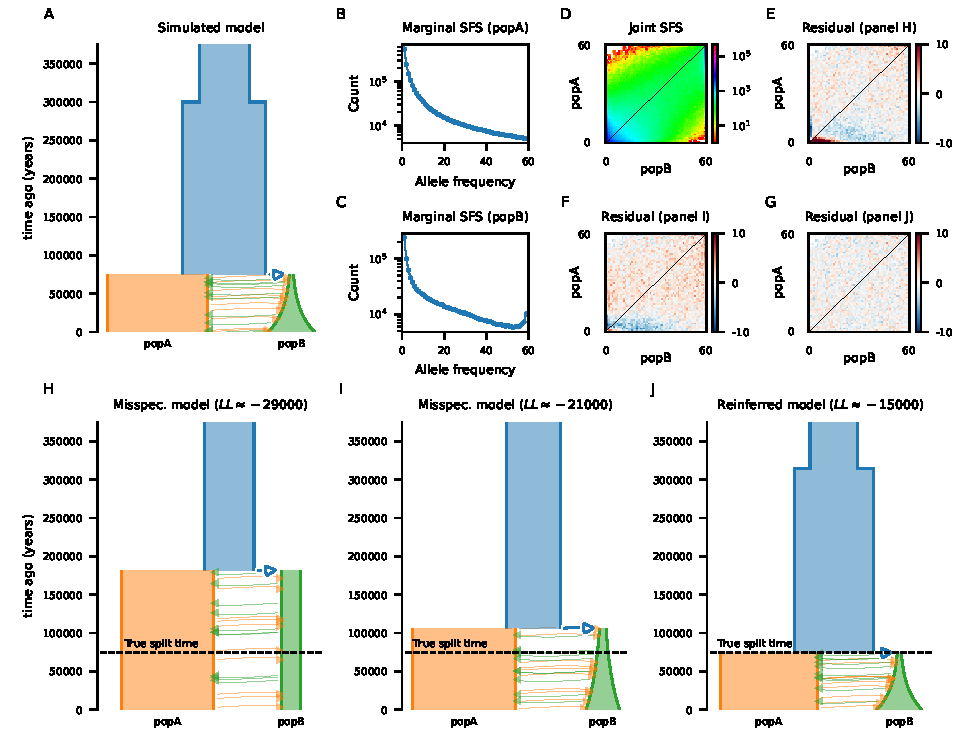
\includegraphics{../example1/fig1.pdf}
    \caption{Caption placeholder}
    \label{fig:im}
\end{figure}

In order to optimize parameters in a \demes model, we need a way to specify
which parameters should be fit. For this, we use a separate YAML-formatted file
to define \texttt{parameters}, each of which points to the value(s) in the
demographic model and sets lower and upper bounds. This file also specifies any
relative \texttt{constraints} between pairs of parameters, to ensure the
optimization routine only explores valid model space. Below, we have included
a truncated parameters file -- the full example is available on GitHub.
\begin{minted}[gobble=4, frame=single]{YAML}
    parameters:
    - name: T0
      values:
      - demes:
          ancestral:
            epochs:
              0: end_time
      lower_bound: 0
      upper_bound: 2e5
    - name: T1
      values:
      - demes:
          ancestral:
            epochs:
              1: end_time
      lower_bound: 0
      upper_bound: 1e6
    - name: Ne
      values:
      - demes:
          ancestral:
            epochs:
              0: start_size
      lower_bound: 1e2
      upper_bound: 1e6
    ...
    constraints:
    - params: [T0, T1]
      constraint: greater_than
\end{minted}

Taking the demographic model, parameters file, and observed SFS together, we
can perform inference using the \texttt{moments.Demes.Inference.optimize(...)}
function.  The initial parameter guesses are given by the input demographic
model, which may be perturbed using a keyword argument. Any value in the
demographic model that is not specified in the parameters file will remain
unchanged, and is therefore treated as a fixed parameter. Here, we also assume
we have an estimate for the total mutation rate, $U$.
\begin{minted}[gobble=4, frame=single]{YAML}
    import moments 

    data = moments.Spectrum.from_file('data.fs')
    U = 1e-8 * 5e8  # per-base mutation rate times the total length

    model_file = 'model.yaml'
    params_file = 'params.yaml'
    output = 'model.fit.yaml'

    ret = moments.Demes.Inference.optimize(
        model_file, params_file, data,
        perturb=1, uL=U, output=output
    )
\end{minted}

Confidence intervals may also be computed, once a (locally) optimal model has
been found.

\subsection*{Inferring parameters in a simulated split-with-migration model}

Using the split-with-migration model defined above (illustrated in
Figure~\ref{fig:im}A), we simulated data for 30 diploid individuals from both
populations using \msprime \citep{baumdicker2022efficient}. These simulations
consided of 500 regions, each of length 1 Mb, with per-base recombination and
mutation rates of $10^{-8}$. The joint SFS was computed using \tskit's
\texttt{ts.allele\_frequency\_spectrum()} function separately on each replicate
region and summing across regions to find the total SFS across 500 Mb of data
(Figure~\ref{fig:im}B--D).

We fit three demographic models to the simulated data. In addition to
reinferring the parameters from the simulated model, we fit two simpler models
to the same data. These had fewer parameters, both omitting the size change
deeper in time in the ancestral population. This is meant to crudely mimic the
scenario that we often face, in which the true history is more complicated than
the parameterized model. It also highlights biases in inferences that can arise
when features of the true history are not included.

When fitting the two misspecified models that do not allow for size changes in
the ancestral population, this split time is inferred to be substantially
deeper in the past than the true split time. This effect, as demonstrated by
\citet{momigliano2020biases}, is due to the decreased coalescence rate within
the ancestral population between the time of the expansion and divergence of
the descendent populations. These two misspecified models
(Figure~\ref{fig:im}H,I) also provide a worse fit to the data, as seen by the
lower log-likelihoods and the large residuals between model predictions and
data (Figure~\ref{fig:im}E-G).

\subsection*{Inferring human-Neanderthal demographic parameters}

\begin{figure}[t!]
    %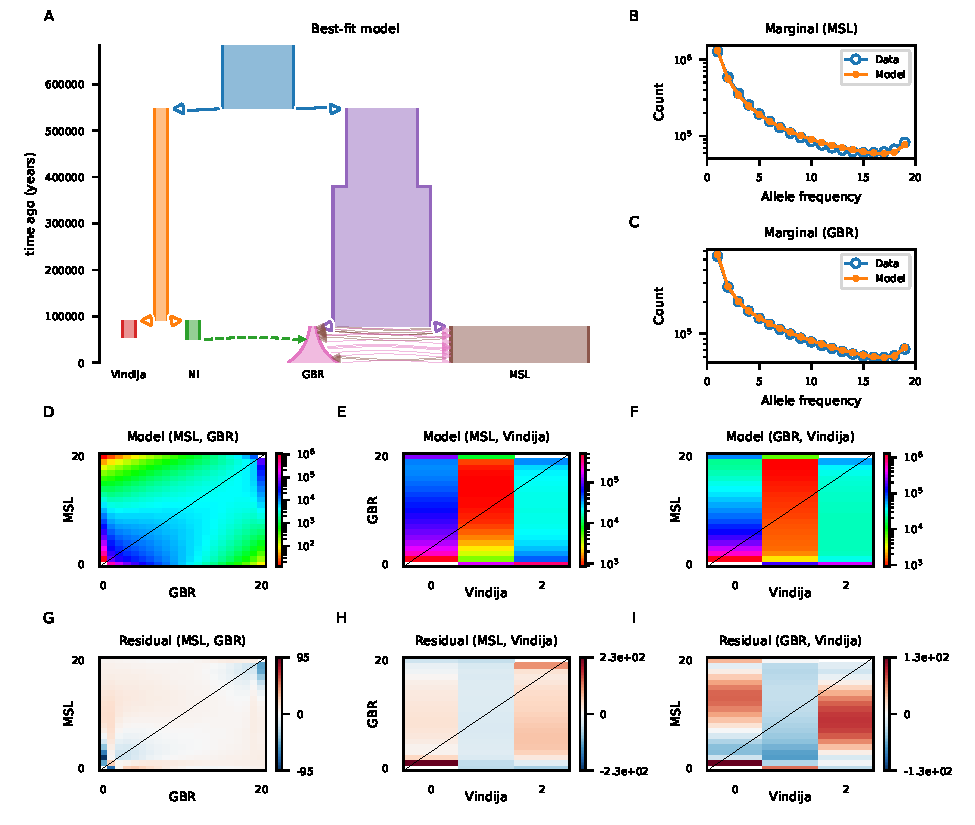
\includegraphics{../example2/fig2.pdf}
    \caption{Caption placeholder}
    \label{fig:humans}
\end{figure}


\section*{Considerations and caveats}\label{sec:conclusions}

\begin{enumerate}
    \item Include here general ideas about the strengths and weaknesses of
        various approaches in population genetic inference, including when
        using the SFS.
    \item Challenges in finding local/global optima.
    \item Challenges in exploring parameter space.
    \item Background selection [Ewing, Johri]
    \item Gene dense vs gene sparse genomic architectures among species.
\end{enumerate}

\bibliographystyle{plainnat}
\bibliography{paper}

\end{document}
